\part{Week 6}
\chapter{Quantum circuits}
\section{Quantum algorithms}
Many interesting problems are impossible to solve on a classical computer, not because they're in principle insoluble, but because of the astronomical amount of resources they'd need. Quantum computing promises to enable feasible algorithms which would require unreasonably high resources for a solution on a classical computer.

As we've discussed before, two broad classes of quantum algorithms exist now, first is based on Shor's \textit{Quantum fourier transform} which provides \textit{exponential} speedup. Second is based on Grover's algorithm for performing \textit{quantum searching} which provides \textit{quadratic} speedup. Few main applications are listed in this figure
\begin{figure}[H]
    \centering
    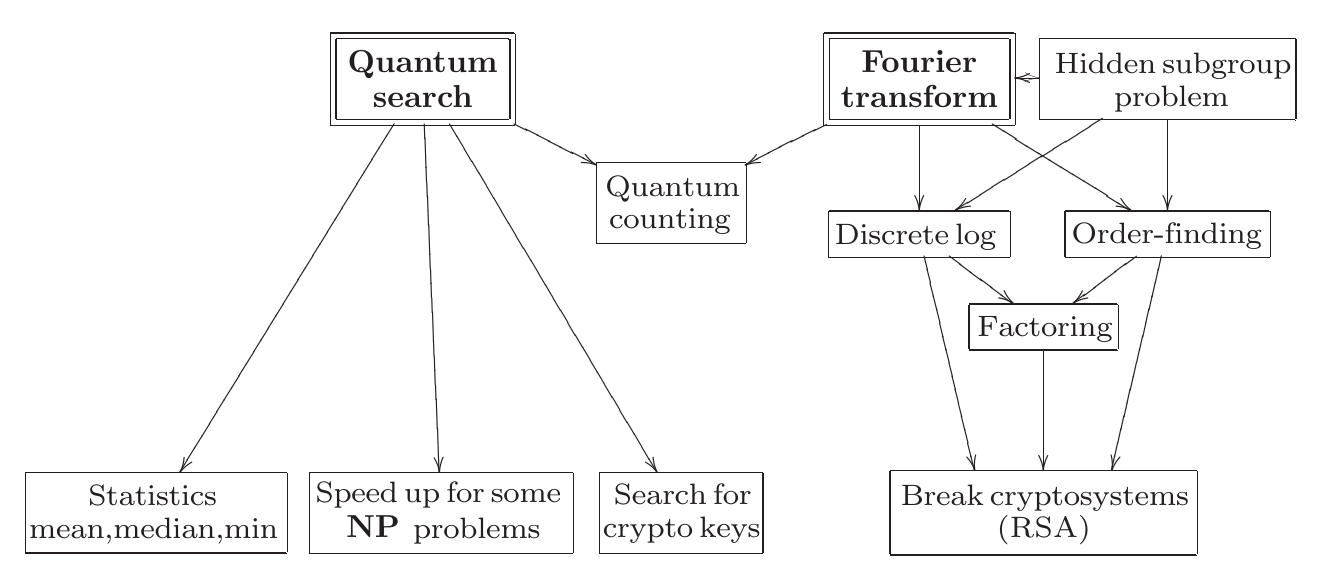
\includegraphics[width=0.9\textwidth]{images/quantum_algorithms.png}
    \caption{Main quantum algorithms with their applications and relationships.}
    \label{fig:quantum-algorithms}
\end{figure}

\section{Single qubit operations}
A single qubit is the simplest quantum system. We already know few important things like norm of the state is 1, operations on it are defined by unitary matrices etc. Few important gates/ operations are Pauli matrices ($I$, $X$, $Y$, $Z$) which we know. Three other important quantum gates are Hadamard gate ($H$), phase gate ($S$), and $\pi/8$ gate ($T$):
\begin{equation}
    H = \frac{1}{\sqrt{2}}\begin{bmatrix}
        1 & 1 \\ 1 & -1
    \end{bmatrix};
    \ \ \ 
    S = \begin{bmatrix}
        1 & 0 \\ 0 & i
    \end{bmatrix};
    \ \ \ 
    T = \begin{bmatrix}
        1 & 0 \\ 0 & \exp{(i\pi/4)}
    \end{bmatrix}.
\end{equation}
Few useful facts are $H = (X+Z)/\sqrt{2}$ and $S=T^2$, $T$ is known as $\pi/8$ gate instead of $\pi/4$ because it's equal to a gate with diagonal $\exp{(\pm \pi/8)}$ upto a global phase factor:
\begin{equation}
    T = \exp{(i\pi/8)}\begin{bmatrix}
        \exp{(-i\pi/8)  } & 0 \\ 0 & \exp{(i\pi/8)}
    \end{bmatrix}
\end{equation}
Also, in \textit{Bloch sphere} representation, the state $a\qo+b\qi$ can be represented as a point $(\theta, \varphi)$ where $a=\cos{(\theta/2)}$ and $b=e^{i\varphi}\sin{(\theta/2)}$, and the Bloch vector is $(\cos{\varphi}\sin{\theta}, \sin{\varphi}\sin{\theta}, \\ \cos{\theta})$.

Pauli matrices give rise to useful matrices when exponentiated, the \textit{rotation operators} about $\hat{x}$, $\hat{y}$ and $\hat{z}$ axes, defined by equations
\begin{align}
    % 1
    R_x(\theta) & \equiv e^{-i\theta X/2} = \cos{\frac{\theta}{2}}I - i\sin{\frac{\theta}{2}}X = \begin{bmatrix}
        \cos{\frac{\theta}{2}} & -i\sin{\frac{\theta}{2}} \\
        -i\sin{\frac{\theta}{2}} & \cos{\frac{\theta}{2}} 
    \end{bmatrix} \\
    % 2
    R_y(\theta) & \equiv e^{-i\theta Y/2} = \cos{\frac{\theta}{2}}I - i\sin{\frac{\theta}{2}}Y = \begin{bmatrix}
        \cos{\frac{\theta}{2}} & -\sin{\frac{\theta}{2}} \\
        \sin{\frac{\theta}{2}} & \cos{\frac{\theta}{2}}
    \end{bmatrix} \\
    % 3
    R_z(\theta) & \equiv e^{-i\theta Z/2} = \cos{\frac{\theta}{2}}I - i\sin{\frac{\theta}{2}}Z = \begin{bmatrix}
        e^{-i\theta/2} & 0 \\
        0 & e^{i\theta/2}
    \end{bmatrix} .
    \end{align}
this is because if $x\in \mathbb{R}$ and $A^2=I$, then $e^{iAx}=\cos{x}I+i\sin{x}A$. If $\hat{n}=(n_x,n_y,n_z)$ is real unit vector in three dimensions then generalize the rotation by $\theta$ about $\hat{n}$ by the equation
\begin{equation}
    R_{\hat{n}}(\theta) = e^{-i\theta \hat{n}\cdot \Vec{\sigma}/2} = \cos{\left( \frac{\theta}{2} \right)}I - \sin{\left( \frac{\theta}{2} \right)}(n_xX+n_yY+n_zZ),
\end{equation}
where $\Vec{\sigma}$ denotes the three component vector $(X, Y, Z)$ of Pauli matrices. A nice fact is that any unitary operator on a single qubit can be written as $U=e^{i\alpha}R_{\hat{n}}(\theta)$ for some $\alpha$, $\hat{n}$ and $\theta$. More generally

\begin{theorem}[\textbf{Z-Y decomposition for a single qubit}]
    Suppose $U$ is a unitary operation on a single qubit. Then there exist real numbers $\alpha$, $\beta$, $\gamma$, $\delta$ such that
    \begin{equation}
        U = e^{i\alpha}R_z(\beta)R_y(\gamma)R_z(\delta)
    \end{equation}
\end{theorem}
In general $z$ and $y$ can be replaced by any non-parallel real unit vectors $\hat{m}$ and $\hat{n}$. Also, this leads to a mysterious corollary, which'll be useful later.
\begin{corollary}
    Suppose $U$ is a unitary gate on a single qubit. Then there exist unitary operators $A$, $B$, and $C$ on a single qubit such that $ABC=I$ and $U=e^{i\alpha}AXBXC$, where $\alpha$ is some overall phase factor.
\end{corollary}
Here are few useful circuit identities:
\begin{equation}
    HXH = Z;\ HYH = -Y;\ HZH = X.
\end{equation}
also, $HTH=R_x(\pi/4)$. To recap things here are few quantum circuit symbols
\begin{figure}[H]
    \centering
    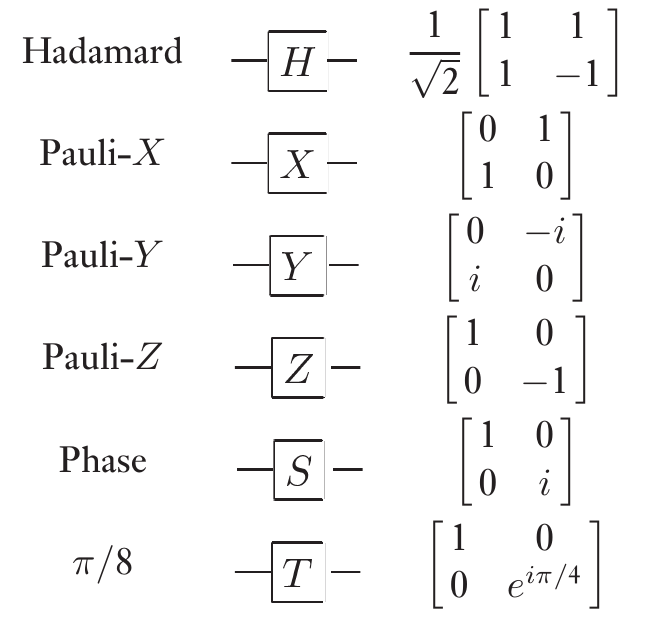
\includegraphics[width=0.4\textwidth]{images/circuit_symbols.png}
    \caption{Names, symbols and unitary matrices for commonly used quantum gates.}
    \label{fig:circuit-symbols}
\end{figure}
\section{Controlled operations}
`If $A$ is true, then do $B$' is the most useful and basic controlled operation in both classical and quantum computation. An example is \textsc{cnot} gate in quantum computation, which does $\ket{c}\ket{t}\rightarrow \ket{c}\ket{t\oplus c}$ where $\ket{c}$ is control qubit and $\ket{t}$ the target qubit. If $\ket{c}$ is in state $\qo$ nothing happens to target qubits, else if it's in $\qi$ $\ket{t}$ is flipped. A general thing for this is \textit{controlled-U} gate, which does $\ket{c}\ket{t}\rightarrow \ket{c}U^c\ket{t}$, where $U$ is a unitary operation. In the computational basis $\ket{\text{control, target}}$, the matrix representation of \textsc{cnot} gate is
\begin{equation}
    \begin{bmatrix}
        1 & 0 & 0 & 0 \\
        0 & 1 & 0 & 0 \\
        0 & 0 & 0 & 1 \\
        0 & 0 & 1 & 0
    \end{bmatrix}.
\end{equation}

To develop \textit{controlled-U} gate for arbitrary $U$, we'll use $U=e^{i\alpha}AXBXC$. To apply the controlled phase shift $\exp{(i\alpha)}$, we use a circuit containing a single qubit gate as shown
\begin{figure}[H]
    \centering
    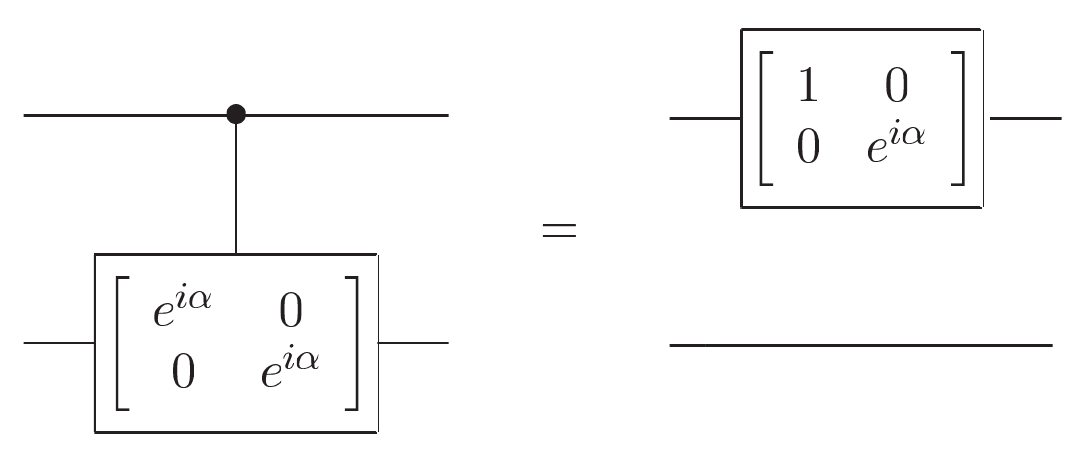
\includegraphics[width=0.5\textwidth]{images/phase_shift_circuit.png}
    \caption{Controlled phase shift gate and an equivalent circuit for two qubits.}
    \label{fig:phase-shift-circuit}
\end{figure}

To complete the gate we use the circuit \ref{fig:controlled-u-circuit}. This works because if control qubit is set to $\qo$ then nothing happens at \textsc{cnot} gates and $ABC=I$ is applied which does nothing, if control qubit is $\qi$ then $e^{i\alpha}AXBXC$ is applied, thus $U$ is applied. 
\begin{figure}[H]
    \centering
    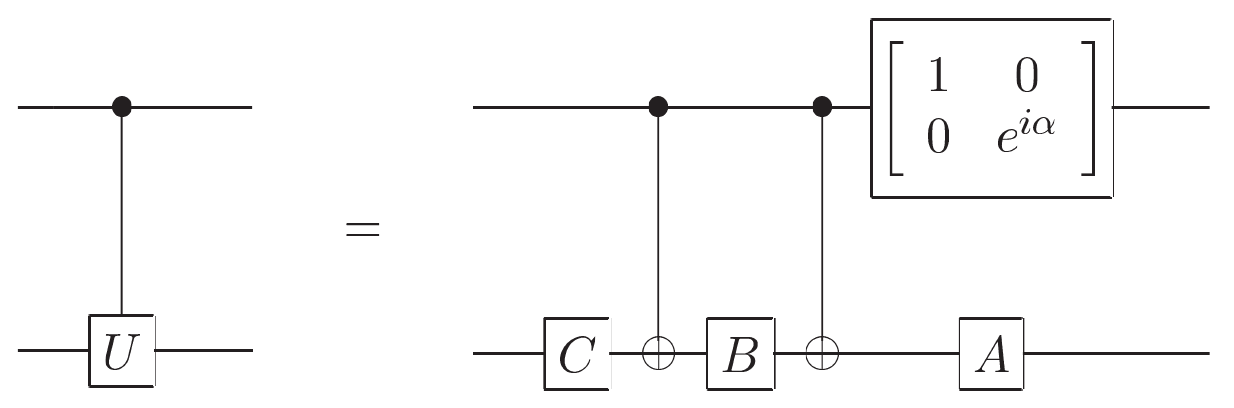
\includegraphics[width=0.7\textwidth]{images/controlled_u_circuit.png}
    \caption{\textit{controlled-U} circuit, $\alpha$, $A$, $B$, $C$ satisfy $U=e^{i\alpha}AXBXC$ and $ABC=I$}
    \label{fig:controlled-u-circuit}
\end{figure}

To use conditioning on multiple-qubits, suppose we have $n+k$ qubits, and $U$ is a $k$ bit operator. Then the controlled operatioin $C^n(U)$ by the equation
\begin{equation}
    C^n(U)\ket{x_1x_2\dots x_n}\qv = \ket{x_1x_2\dots x_n}U^{x_1x_2\dots x_n}\qv
\end{equation}
where $x_1x_2\dots x_n$ means product of those bits. It means operation $U$ is applied on last $k$ qubits if all of the first $n$ qubits are $\qi$. We'd assume $k=1$, for $k\geq2$ we don't yet know how to perform $k$ arbitrary operations at once.
\begin{figure}[H]
    \centering
    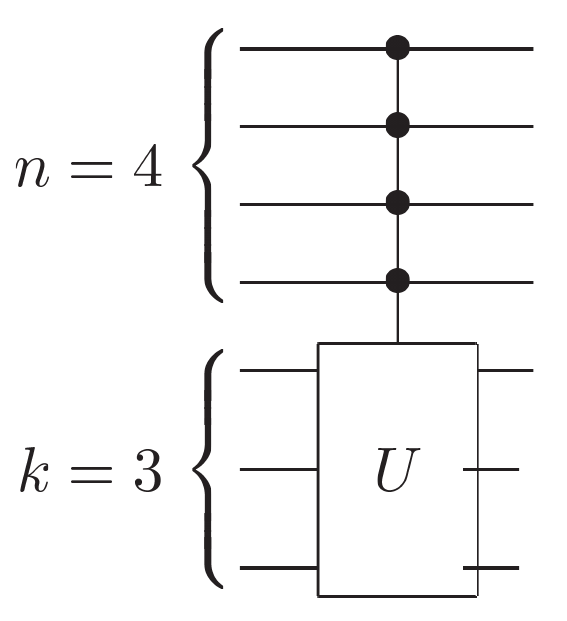
\includegraphics[width=0.4\textwidth]{images/multi_qubit_operation_circuit.png}
    \caption{$C^n(U)$ operation for $n=4$ and $k=3$.}
    \label{fig:multi-qubit-operation}
\end{figure}

\begin{figure}[H]
    \centering
    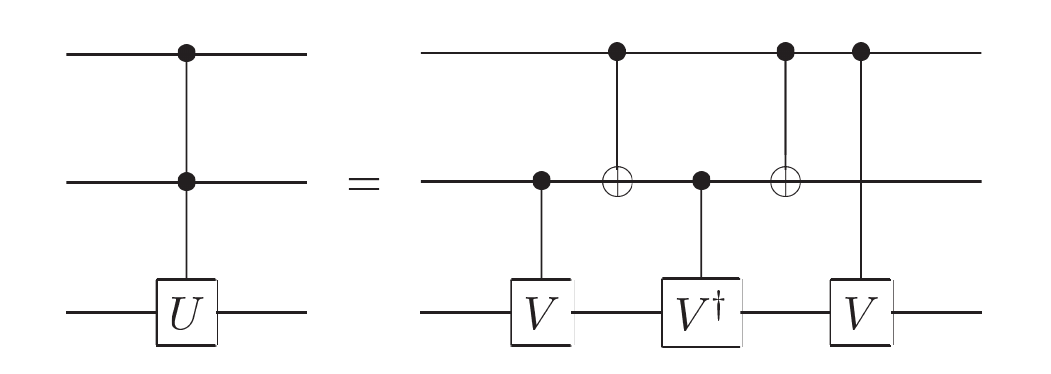
\includegraphics[width=0.8\textwidth]{images/c2u_gate.png}
    \caption{$C^2(U)$ gate. $V$ is a unitary operator satisfying $V^2=U$. When $V\equiv (1-i)(1+iX)/2$ represents the Toffoli gate.}
    \label{fig:c2u}
\end{figure}
Remember that when $U=X$, $C^2(U)$ is known as the \textit{Toffoli gate}.

How $C^n(U)$ is implemented is interesting, first we take the first $n$ qubits as $\ket{c_1},\ket{c_2}\dots \\ \ket{c_n}$, we use $(n-1)$ intermediate working qubits which are all initially and finally $\qo$, which store $\ket{c_1c_2},\ket{c_1c_2c_3}\dots \ket{c_1c_2\dots c_n}$. This is done using toffoli gates which is applied between $\ket{c_1}$ and $\ket{c_2}$ with the output to first working qubit, the next toffoli gate is applied between first working qubit and $\ket{c_3}$ which gives $\ket{c_1c_2c_3}$ and so on, thus giving $\ket{c_1c_2\dots c_n}$.

\begin{figure}[H]
    \centering
    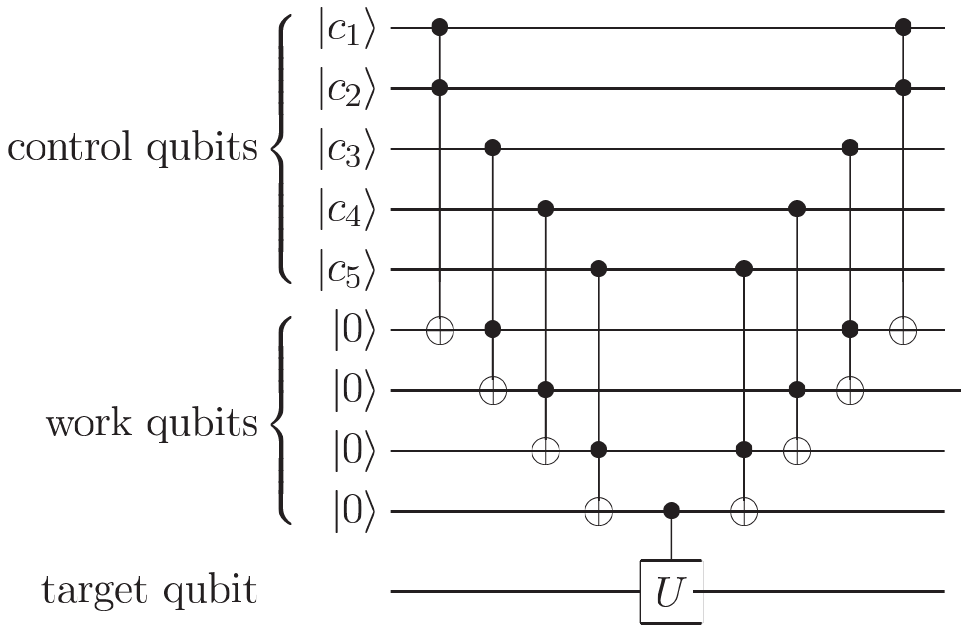
\includegraphics[width=0.65\textwidth]{images/c_n_u_implementation.png}
    \caption{Implementation of $C^n(U)$ circuit.}
    \label{fig:c-n-u-implementation}
\end{figure}

We are considering conditionals being $1$ till now, but sometimes it's useful to keep the conditional as $0$ for which we introduce a notation, we keep an open circle (without darkening it) whereas we used to have a darkened circle till now.
\begin{figure}[H]
    \centering
    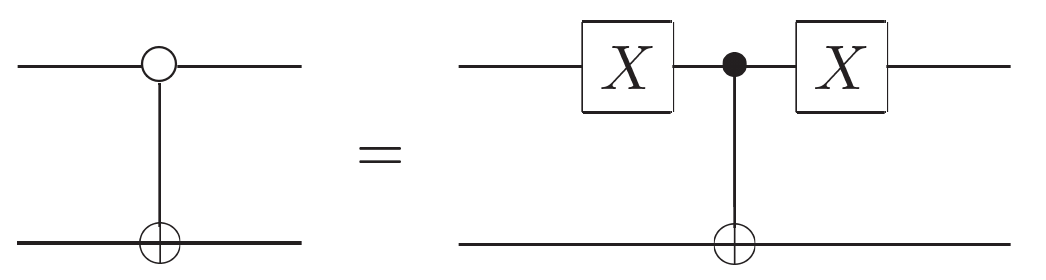
\includegraphics[width=0.75\textwidth]{images/0_notation.png}
    \caption{\sc{cnot} gate, with the conditional being that first qubit is set to $0$.}
    \label{fig:0-notation}
\end{figure}

\section{Measurement}
As we've shown before measurements will be shown by a `meter' symbol, especially projective measurements. There are two major principles worth emphasizing early, first is that classically conditioned operations can be replaced by quantum controlled operations:
\\
\begin{addmargin}[2em]{2em}
    \textbf{Principle of deferred measurement:} Measurements can always be moved from an intermediate state of a quantum circuit to the end of the circuit; if the measurement results are used at any stage, then the classically conditioned operations can be replaced by conditional quantum operations. \\
\end{addmargin}
\begin{addmargin}[2em]{2em}
    \textbf{Principle of implicit measurement:} Without loss of generality, any unterminated quantum wires (qubits which are not measured) at the end of a quantum circuit may be assumed to be measured.
\end{addmargin}

\section{Universal quantum gates}
If a set of gates can compute any arbitrary classical function, they are said to bee \textit{universal} for classical computation. Toffoli gate is universal for classical computation, hence quantum computation subsumes classical conputation.
\subsection{Two level unitary gates are universal}
We'll see how to decompose a $d$-dimensional unitary matrix $U$ into a product of \textit{two-level unitary matrices}, which act non-trivially on only two or fewer components. We'll understand what're these by going forward. Let's take an example $U$ where it's $3\times3$,
\begin{equation}
    U = \begin{bmatrix}
        a & d & g \\
        b & e & h \\
        c & f & i \\
    \end{bmatrix}.
\end{equation}
We can find two-level unitary matrices such that
\begin{equation}
    U_3U_2U_1U = I
\end{equation}
or, $U=U_1^\dag U_2^\dag U_3^\dag$. More generally, for $d$-dimensional space, $U$ can be written as
\begin{equation}
    U = V_1\cdots V_k
\end{equation}
where the matrices $V_i$ are unitary matrices and $k\leq (d-1) + (d-2) + \dots + 1 = d(d-1)/2$. This follows that any unitary operator on $n$ qubits can be written as a product of $2^{n-1}(2^n-1)$ two-level unitary matrices.

\subsection{A discrete set of universal operators}
\subsubsection{Approximating unitary operators}
A \textit{discrete} set of gates can't describe any unitary operator, since the latter are continuous. Suppose we want to implement operator $U$ but what we actually implement is $V$, the \textit{error} when $V$ is implemented instead of $U$ is
\begin{equation}
    E(U,V) \equiv \max_{\qv}||(U-V)\qv||
\end{equation}
maximum is over all  normalized states $\qv$ of state space.
\subsubsection{Universality of Hadamard + phase + \textsc{cnot} + $\pi/8$ gates}
We're going to study two different discrete set of gates, both of which are universal. \textit{Standard set} consists of Hadamard, \textsc{cnot} and $\pi/8$ gates. The second set of gates contains Hadamard, phase, \textsc{cnot} and Toffoli gates. All of these gates can be done fault tolerantly. 

It can be shown that using these gates, any rotation can be done up to desired accuracy. Given any single qubit operator $U$ and any $\epsilon>0$ it's possible to approximate $U$ within $\epsilon$ using a circuit composed of Hadamard and $\pi/8$ gates alone. This simulation is efficient, because the overhead required to perform the simulation is polynomial in $\log(m/\epsilon)$, where $m$ is number of gates in circuit and $\epsilon$ is desired accuracy.

\subsection{Approximating arbitrary unitary gates is generically hard}
There are states of $n$ qubits which take $\Omega(2^n\log(1/\epsilon)/\log(n))$ operations to approximate to within a distance $\epsilon$. This is exponential in $n$, and thus is 'difficult'. This implies that there are unitary transformations $U$ on $n$ qubits which take $\Omega(2^n\log(1/\epsilon)/\log(n))$ operations to approximate by a quantum circuit implementing an operation $V$ such that $E(U,V) \leq \epsilon$.
\section{Simulation of quantum systems}
To simulate, solutions of differential equations capturing physical laws governing the dynamical behaviour of the system. For example the Newton's law,
\begin{equation}
    \frac{d}{dt}\left(m\frac{dx}{dt}\right) = F,
\end{equation}
Poisson's equation,
\begin{equation}
    -\Vec{\nabla}\cdot(k\Vec{\nabla}\Vec{u}) = \Vec{Q},
\end{equation}
the electromagnetic vector wave equation,
\begin{equation}
    \Vec{\nabla}\cdot\Vec{\nabla}\Vec{E} = \epsilon_0\mu_0\frac{\partial^2\Vec{E}}{\partial t^2},
\end{equation}
and the diffusion equation,
\begin{equation}
    \Vec{\nabla}^2\psi = \frac{1}{a^2} \frac{\partial \psi}{\partial t},
\end{equation}
Solutions for these are obtained by using \textit{approximation}. However simulation of quantum systems by classical computers is inefficient. Many simple quantum systems are governed by
\begin{equation}
    i\hbar\frac{d}{dt}\qv = H\qv.
\end{equation}
For a Hamiltonian dealing with particles in space, this reduces to
\begin{equation}
    i\frac{\partial}{\partial x}\psi(x) = \left[-\frac{1}{2m}\frac{\partial^2}{\partial x^2} + V(x)\right] \psi(x),
\end{equation}
using a convention known as the position representation $\braket{x|\psi} = \psi(x)$. The key challenge is there \textit{exponential} number of differential equations to be solved. For $n$ qubits, $2^n$ equations.

Quantum computers can efficiently simulate quantum systems for which there is no known efficient classical simulation. This is similar to the fact that any quantum circuit can be designed from a discrete set of gates. Ofcourse, there are few operators which can't be efficiently approximated, similarly there are few systems with Hamiltonians which can't be efficiently simulated on a quantum computer.

\subsection{The quantum simulation algorithm}
Similar to how we use $y(t+\Delta t) \approx y(t)+f(y)\Delta t$ to solve $dy/dt=f(y)$. To solve $id\qv/dt = H\qv$, which for time independent $H$ is,
\begin{equation}
    \ket{\psi(t)} = e^{-iHt}\ket{\psi(0)}.
\end{equation}
Similarly, exponentiating $H$ would be very inefficient, thus we use $\ket{\psi(t+\Delta t)}
\approx (I-iH\Delta t)\ket{\psi(t)}$. However this isn't very satisfactory. But this can be improved by writing it as a sum of Hamiltonians acting on fewer qubits.

The heart of quantum simulation algorithms is the following asymptotic approximation theorem:
\begin{theorem}[\textbf{Trotter formula}]
    Let $A$ and $B$ be Hermitian operators. Then for any real $t$,
    \begin{equation}
        \lim_{n\rightarrow\infty}(e^{iAt/n}e^{iBt/n})^n = e^{i(A+B)t}.
    \end{equation}
\end{theorem}
Here's an overview of quantum simulation algorithm,

\begin{algorithm}
     \SetAlgoLined\DontPrintSemicolon
    \caption{Quantum simulation}
    \SetKwInOut{KwIn}{Inputs}
    \SetKwInOut{KwOut}{Outputs}
    \SetKwInOut{KwRun}{Runtime}
    \SetKwProg{myprog}{Procedure}{}{}

    \KwIn{
        (1) A Hamiltonian $H=\sum_kH_k$ acting on an $N$-dimensional system, where each $H_k$ acts on a small subsystem of size independent of $N$, (2) an initial state $\ket{\psi_0}$, of the system at $t=0$, (3) a positive, non-zero accuracy $\delta$, and (4) a time $t_f$ at which the evolved state is desired.
    }
    \KwOut{
        A state $\ket{\Tilde{\psi}(t_f)}$ such that 
        $|\braket{\Tilde{\psi}(t_f)|e^{-iHt_f}|\psi_0}|^2 \geq 1-\delta$.
    }
    \KwRun{
        $O(\text{poly}(1/\delta))$ operations.
    }
    \myprog{}{
        Choose a representation such that the state $\ket{\Tilde{\psi}}$ of $n=\text{poly}(\log{N})$ qubits approximates the system and the operators $e^{-iH_k\Delta t}$ have efficient quantum circuit approximations. Select an approximation method and $\Delta t$ such that the expected error is      acceptable (and $j\Delta t=t_f$ for an integer $j$), construct the corresponding quantum circuit $U_{\Delta t}$ for the iterative step, and do:\;
        $\ket{\Tilde{\psi_0}} \leftarrow \ket{\psi_0};\ j=0$ \tcp*{initialize state}\;
        $\rightarrow \ket{\Tilde{\psi_{j+1}}} = U_{\Delta t}\ket{\Tilde{\psi_j}}$\tcp*{iterative update}\;
        $\rightarrow j=j+1; \text{ goto step 2 until } j\Delta t \geq t_f$ \tcp*{loop}\;
        $\rightarrow \ket{\Tilde{\psi}(t_f} = \ket{\Tilde{\psi_j}}$ \tcp*{final result}
    }
\end{algorithm}